\section*{Learning Objectives}

\begin{itemize}
\item How to efficiently compute derivatives and partial derivatives of functions.
\item Remove a common source of errors in Engineering: doing Calculus by hand!
\end{itemize}

\section*{Outcomes} 
\begin{itemize}
\item Symbolic computations in Julia

\item Numerical derivatives in Julia

\item Automatic Differentiation, the current workhorse for Machine Learning
\end{itemize}

\vspace*{1cm}

\textbf{Either download Lab10 from our Canvas site or open up a Jupyter notebook so that you can enter code as we go. It is suggested that you have line numbering toggled on.}  

\begin{figure}
    \centering
    
\includegraphics[width=0.7\columnwidth]{graphics/Chap10/AutomaticDifferentiationChiFengWang.jpeg}
    \caption{
   \url{https://towardsdatascience.com/automatic-differentiation-explained-b4ba8e60c2ad}
    } is the source of the image.
    \label{fig:my_label}
\end{figure}

\newpage

The material in this Chapter/Lab is due to Alphonsus Antwi Adu-Bredu, who was the lead GSI for ROB 101 in F-22, while he was also a Ph.D. candidate in Robotics. Here are the key packages we will use. \\

\begin{lstlisting}[language=Julia,style=mystyle]
# Let's install some Julia packages. 
using Pkg
Pkg.add("Symbolics")
Pkg.add("FiniteDiff")
Pkg.add("ForwardDiff")
Pkg.add("BenchmarkTools");
\end{lstlisting}
\textbf{Output} 
\begin{verbatim}
Nothing.
\end{verbatim}

\section{Symbolic Differentiation}

This is the kind of differentiation you learned (or will learn) in your intro Calculus classes. Using this approach, you can take derivatives of expressions using the various rules of differential calculus, such as 
\begin{itemize}
    \item $\frac{d}{d x} c = 0 $, where c is a constant
\item $\frac{d}{d x} x = 1 $
\item $\frac{d}{d x} y = 0 $, where $y$ is a variable other than $x$
\item $\frac{d}{dx} (u + v) = \frac{d}{d x} u + \frac{d}{d x} v = 0 $
\item $\frac{d}{d x} (u \cdot v) = u \cdot \frac{d}{d x} v + v \cdot \frac{d}{d x} u $ 
\item $\frac{d}{d x} \frac{u}{v} = \frac{(v \cdot \frac{d}{d x}u -  u \cdot \frac{d}{dl x} v)}{v^2}$
\item Etc. $\dots$
\end{itemize}

This form of differentiation is called symbolic, because it allows you to perform differentiation by manipulating symbols, or more precisely, variables, without actually evaluating them as real numbers. This is a big part of Calc I. As you may have guessed, Julia has a sweet package called \texttt{Symbolics.jl} which allows you to take symbolic derivatives of input expressions. The next few cells will teach you how to use this package.\\

\textbf{Example 1:} Find the derivative of the function 
$$f(x) = x^3cos(x) + x^2sin(x)^2 + log(3x)$$
using Symbolic Differentiation. \\

Step 1: We load the Symbolics.jl package. Just like any other Julia packages used in this course, loading Symbolics.jl for the first time often takes a while.

\begin{lstlisting}[language=Julia,style=mystyle]
 using Symbolics
\end{lstlisting}

Step 2: We declare the variables in our function using the \texttt{@variables} macro. The only variable in the function above is $x$.

\begin{lstlisting}[language=Julia,style=mystyle]
@variables x
\end{lstlisting}
\textbf{Output} 
\begin{verbatim}
[x]
\end{verbatim}

Step3: We create the differential operator $\frac{d}{d x}$ and assign it to a variable. 

\begin{lstlisting}[language=Julia,style=mystyle]
d/dx = Differential(x)
\end{lstlisting}
\textbf{Output} 
\begin{verbatim}
(::Differential) (generic function with 2 methods)
\end{verbatim}

Step 4: We define $f(x)$ and apply our differential operator  $\frac{d}{d x}$ to it. 

A cool feature about \texttt{Symbolics.jl} is that it renders our expressions in Latex in the cell outputs!
\begin{lstlisting}[language=Julia,style=mystyle]
f = x^3*cos(x) + x^2*sin(x)^2 + log(3x)
d/dx(f)
\end{lstlisting}
\textbf{Output} \\
$\mathrm{\frac{d}{d x}}\left( \sin^{2}\left( x \right) x^{2} + x^{3} \cos\left( x \right) + \log\left( 3 x \right) \right)$\\

Step 5: We compute the derivative $\frac{d f}{d x}$  using the \texttt{expand\_derivatives} function and store it in variable $\Delta f$. The derivative expression is printed out in the cell output.

\begin{lstlisting}[language=Julia,style=mystyle]
dfdx = expand_derivatives(d/dx(f)) 
\end{lstlisting}
\textbf{Output} \\
$x^{-1} + 2 \sin^{2}\left( x \right) x - x^{3} \sin\left( x \right) + 3 x^{2} \cos\left( x \right) + 2 x^{2} \cos\left( x \right) \sin\left( x \right)$\\

\textbf{Simpler, alternative formulation:} We use the \texttt{Symbolics.derivative} function to directly compute derivatives of $f$

\begin{lstlisting}[language=Julia,style=mystyle]
dfdx = Symbolics.derivative(f, x)
\end{lstlisting}
\textbf{Output} \\
$\mathrm{\frac{d}{d x}}\left( \sin^{2}\left( x \right) x^{2} + x^{3} \cos\left( x \right) + \log\left( 3 x \right) \right)$

\begin{tcolorbox}
    Remark: We are not restricted to derivatives of scalar-valued functions. We can also use \texttt{Symbolics.jl} to compute gradients, Jacobians, and Hessians of multivariate functions. The following cells show how to get the actual latex code

    \begin{lstlisting}[language=Julia,style=mystyle]
# This cell shows how to get the actual latex code
using Latexify
set_default(fmt = "%.0f", convert_unicode = false)
latexify(d/dx(f)) |> print
\end{lstlisting}
\textbf{Output} 
\begin{verbatim}
\begin{equation}
\mathrm{\frac{d}{d x}}\left( \sin^{2}\left( x \right) x^{2} 
+ x^{3} \cos\left( x \right) + \log\left( 3 x \right) \right)
\end{equation}
\end{verbatim}
$\mathrm{\frac{d}{d x}}\left( \sin^{2}\left( x \right) x^{2} 
+ x^{3} \cos\left( x \right) + \log\left( 3 x \right) \right)$

Note that \texttt{fmt = "\%.0f"} and \texttt{fmt = "\%.4f"} set the formatting for numbers in the expressions.
\begin{lstlisting}[language=Julia,style=mystyle]
# This cell shows how to get the actual latex code
using Latexify
set_default(fmt = "%.4f", convert_unicode = false)
latexify(d/dx(f)) |> print
\end{lstlisting}
\textbf{Output} 
\begin{verbatim}
\begin{equation}
\mathrm{\frac{d}{d x}}\left( \sin^{2.0000}\left( x \right) x^{2.0000} + 
x^{3.0000} \cos\left( x \right) + \log\left( 3.0000 x \right) \right)
\end{equation}
\end{verbatim}
$\mathrm{\frac{d}{d x}}\left( \sin^{2.0000}\left( x \right) x^{2.0000} + x^{3.0000} \cos\left( x \right) + \log\left( 3.0000 x \right) \right)
$

\end{tcolorbox}

If we later want to evaluate this derivative expression at some numerical value, we can use the \texttt{substitute} function, which takes as arguments, the computed derivative expression as well as a ``dictionary'' that maps variables to their desired values. Here, our desired value for $x$ is 0.5 . The value of our derivative at this value of $x$ is 3.0384753223601586

\begin{lstlisting}[language=Julia,style=mystyle]
val = substitute(dfdx, (Dict(x=>0.5)))
\end{lstlisting}
\textbf{Output} 
\begin{verbatim}
3.038475322360
\end{verbatim}

\begin{center} 
\textbf{Advantages and Disadvantages of Symbolic Differentiation}
\end{center}



\begin{itemize}
    \item \textcolor{blue}{\bf Advantage:} Symbolic Differentiation allows you to compute exact derivatives up to machine precision.
    \item \textcolor{blue}{\bf Advantage:} Symbolic Differentiation is also a great tool for analysis. Being able to generate closed-form derivatives of a dynamical model of a robot facilitates the understanding of the dynamics of the robot.
    \item \textcolor{blue}{\bf Advantage:} Symbolic Differentiation is also significantly useful for generating closed-form derivatives of functions as code. Closed-loop controllers running on real-time systems often have to run at frequencies in the 1kHz range. This constrains the control loop to a time budget of 1 millisecond. Given this time budget, operations in the controller (such as computing derivatives and Jacobians) have to be as fast as possible. Closed-form parameterized functions for derivatives and Jacobians that are computed offline using Symbolic differentiation can then be evaluated online in microseconds, which can be very useful in speeding up your controller and meeting the controller time budget.

    \item \textcolor{red}{\bf Disadvantage:} The main disadvantage of symbolic derivatives is that they tend to get gnarly and exponentially long very quickly. This phenomenon is called \textbf{Expression swell}. 
    \item \textcolor{red}{\bf Disadvantage:} Imagine taking the derivative of a function $h(x) = f(x)g(x)$, where $f(x)$ is itself the product $f(x) = u(x)v(x)$. The derivative of $h(x)$ ends up as this gnarly function $$\frac{d}{dx}h(x) = \Bigg(\frac{d}{dx}u(x)v(x) + u(x)\frac{d}{dx}v(x)\Bigg)g(x) + u(x)v(x)\frac{d}{dx}g(x)$$  leading to inefficient code.
\end{itemize}

\section{Numerical Differentiation}

Numerical differentiation is another approach for taking derivatives of functions. Unlike Symbolic differentiation, where we derive exact, analytical derivatives of functions, numerical differentiation estimates the derivatives of functions using values of the function at various points. \\

The simplest and most common method for Numerical Differentiation is \textbf{Finite Difference}, as we have used in ROB 101 for building linear approximations of nonlinear functions.\\

The method of finite differences approximates the derivative $\frac{d f(x_0)}{d x}$ of a function $f$ at some (numerical) point $x_0$ as $$\frac{d f(x_0)}{d x} = \frac{f(x_0+h) - f(x_0)}{h}.$$ This specific finite difference is specifically known as the \textbf{Forward Difference} approximation. There also exists a \textbf{Backward Difference} approximation, which is expressed as $$\frac{d f(x_0)}{d x} = \frac{f(x_0) - f(x_0-h)}{h}$$ and a \textbf{Symmetric Difference} approximation expressed as $$\frac{d f(x_0)}{d x} = \frac{f(x_0+h) - f(x_0-h)}{2h}.$$ If the derivative of $f(x)$ exists at a point $x_0$, for some small $h$, the forward, backward and symmetric difference approximations are approximately equal. If they end up being significantly different, then the function $f(x)$ is not differentiable at $x_0$.\\

As you may have guessed by now, there exists a really sweet Julia package with implementations of finite differences called \texttt{FiniteDiff.jl}, which in fact has empirically the fastest implementation of finite differences in any programming language! \\

In the following cells, we are going to learn how to use it to take derivatives, gradients, Jacobians, and Hessians of functions. The main difference between derivatives and gradients in relation to the \texttt{FiniteDiff.jl} package is that derivatives are used for functions depending on a scalar $x\in \real$ while gradients are used for functions depending on a vector of variables.\\

\textbf{Example 2:} Find the derivative $\frac{d g(x)}{d x}$ of the function 
$$g(x) = x^3cos(x) + x^2sin(x)^2 + log(3x)$$ using Finite Differences.

\begin{lstlisting}[language=Julia,style=mystyle]
using FiniteDiff 

g(x) = x^3 ~cos(x) + x^2~sin(x)^2 + log(3x)
\end{lstlisting}
\textbf{Output} 
\begin{verbatim}
g (generic function with 1 method)
\end{verbatim}

To compute the derivative of the function $g(x($ at $x_0=0.5$, we use the function \texttt{FiniteDiff.finite\_difference\_derivative}. The first argument of the function is $g(x)$, the function whose derivative is to be taken, and the second argument is the point at which the derivative is to be taken. Note that we obtain a solution that is approximately equal to that of the Symbolic derivative in the previous section.

\begin{lstlisting}[language=Julia,style=mystyle]
val = FiniteDiff.finite_difference_derivative(g, 0.5)
\end{lstlisting}
\textbf{Output} 
\begin{verbatim}
3.038475322499568
\end{verbatim}

\textbf{Example 3:} Compute the Jacobian of the function 
$$ h(x) = \begin{bmatrix} x_1^3cos(x_2) + x_2^2sin(x_1)^2 \\
      log(3x_3) \end{bmatrix}$$ 
using Finite Differences,
where $x \in \mathbb{R}^3$ and $x_i$ is the $i$-{th} element of $x$.

\begin{lstlisting}[language=Julia,style=mystyle]
h(x) = [x[1]^3*cos(x[2]) + x[2]^2*sin(x[1])^2;
                        log(3x[3])]

x0 = [0.1, 0.5, 0.7]
J = FiniteDiff.finite_difference_jacobian(h, x0)
\end{lstlisting}
\textbf{Output} 
\begin{verbatim}
2x3 Matrix{Float64}:
 0.0759948  0.00948729  0.0
 0.0        0.0         1.42857
\end{verbatim}

And the \textbf{Hessian} of the super complicated function
$$h_2(x) = x^\top A_2 x + x^\top xx^\top A_4 x$$
can be computed as

\begin{lstlisting}[language=Julia,style=mystyle]
using Random
n=3
A2 = rand(n,n) 
A4 = rand(n,n)
h2(x)= x'*A2*x + x'*x*x'*A4*x;
x0 = [0.1, 0.5, 0.7]
H = FiniteDiff.finite_difference_hessian(h2, x0)
\end{lstlisting}
\textbf{Output} 
\begin{verbatim}
3x3 LinearAlgebra.Symmetric{Float64, Matrix{Float64}}:
 3.12914  3.32833  2.95256
 3.32833  5.92296  4.11562
 2.95256  4.11562  5.5207
\end{verbatim}

\begin{center}
\bf Advantages and Disadvantages of Numerical Differentiation
\end{center}

\begin{itemize}
    \item \textcolor{blue}{\bf Advantage:} Numerical differentiation is the simplest differentiation method to implement. It only depends on the function values and not on a set of differential calculus rules.
 In view of this, numerical differentiation can be applied to any differentiable function to get reasonably accurate results.

    \item \textcolor{red}{\bf Disadvantage:} Finite Difference suffers from \textbf{Truncation error}, resulting in inaccurate derivatives when the step size is too big or too small.

 \item \textcolor{red}{\bf Disadvantage:} Finite Difference can also be expensive to compute for functions with large input dimensions.
\end{itemize}

\section{Automatic Differentiation}

Similar to Symbolic Differentiation, \texttt{Automatic Differentiation} uses a set of rules from differential calculus to compute derivatives. However, its goal is to return a numerical solution instead of a closed-form analytical expression. As such, \texttt{Automatic Differentiation} keeps track of intermediate variables and their derivatives to speed up computation. It decomposes the function into primitive operations using the chain rule, evaluates the operations and their derivatives, and stores them in intermediate variables; see \url{https://julia.quantecon.org/more_julia/optimization_solver_packages.html}\\

To appreciate how automatic differentiation works, let's take a look at an example. We would like to compute the Jacobian of the multivariate function $$f(x,y) = y\cdot sin(x) + y^2$$ at a point $x=0.1, y=0.3$ using automatic differentiation.\\

We define the $(^\bullet)_x$ operator as the partial derivative with respect to $x$, that is, $\frac{\partial}{\partial x}$. The notation $\dot{a}$ for the derivative is due to Isaac Newton \url{https://en.wikipedia.org/wiki/Notation_for_differentiation}. Next, we decompose $f(x,y)$ into primitive operations and store their values and derivatives with respect to $x$ in intermediate variables. \\

	\centerline{ \fbox{ 
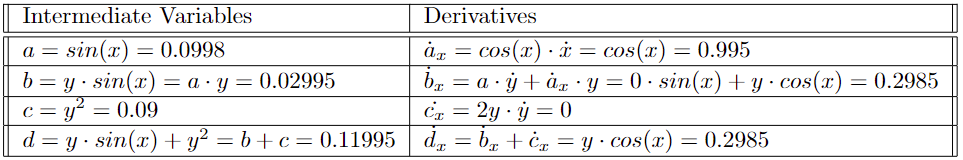
\includegraphics[width=0.9\columnwidth]{graphics/Chap10/AutoDiffImage01.png}}%
}

\vspace*{.2cm}

This routine is called a \textbf{forward pass} with respect to x. It is worth noting that, unlike symbolic differentiation, the numerical values of each intermediate variable are computed in each row of the table. \\

Similarly, we define the $(^\bullet)_y$ operator as the partial derivative with respect to $y$,  $\frac{\partial}{\partial y}$, and define the intermediate variables and derivatives with respect to $y$\\

	\centerline{ \fbox{ 
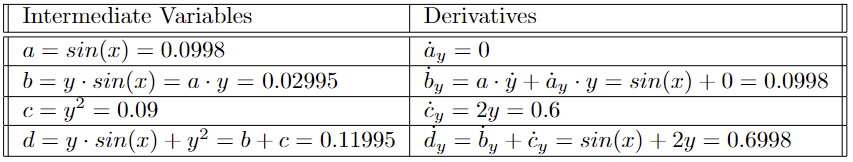
\includegraphics[width=0.9\columnwidth]{graphics/Chap10/AutoDiffImage02.png}}%
}

\vspace*{.2cm}

The Jacobian of $f(x,y)$ can now be defined as $$Jac = \frac{\partial f(x,y)}{\partial (x, y)} = [\dot{d}_x~~~\dot{d}_y] = [0.2985 ~~~ 0.6998]$$
The computational routine we have just demonstrated above is a special kind of Automatic Differentiation called \textbf{Forward-Mode Automatic Differentiation}. \\

In general, you would perform a forward pass for each argument to your function $f$. If the function argument is a vector, you would perform a forward pass for each element in the vector. The computational complexity is of the order $O(n)$. You can imagine that this could end up being computationally inefficient for functions $f : \mathbb{R}^n \rightarrow \mathbb{R}^m$ with $n >>> m$. In such cases, another special kind of Automatic Differentiation called \textbf{Reverse-mode Automatic Differentiation} will be much more appropriate. \\

Reverse-mode Automatic Differentiation first performs a forward pass to compute only the intermediate variable values without taking the derivatives. It then performs a reverse (backward) pass to compute the derivatives of the intermediate variables. A function $f : \mathbb{R}^n \rightarrow \mathbb{R}^m$, will require $m$ reverse passes to compute the Jacobian of the function. Because of this, Reverse-Mode automatic differentiation is suitable for functions where $n >>> m$ and inefficient for functions where $m >>> n$.\\

As you may rightly guess, Julia has packages that have super-fast implementations of forward-mode and reverse-mode automatic differentiation named \texttt{ForwardDiff.jl} and \texttt{ReverseDiff.jl}. In the following cells, we will demonstrate the usage of \texttt{ForwardDiff.jl} for computing derivatives and Jacobians.\\

\textbf{Example 4:} Find the derivative $\frac{d f_2}{d x}$ of the function 
$$f_2(x) = x^3cos(x) + x^2sin(x)^2 + log(3x)$$ using Forward-mode Automatic Differentiation.

\begin{lstlisting}[language=Julia,style=mystyle]
using ForwardDiff
#
f_2(x) = x^3*cos(x) + x^2*sin(x)^2 + log(3x)
\end{lstlisting}
\textbf{Output} 
\begin{verbatim}
f_2 (generic function with 1 method)
\end{verbatim}

Next, we will evaluate the derivative of our function at the point x=0.5 using the function \texttt{ForwardDiff.derivative}. The first argument is the function whose derivative is to be taken, while the second argument is the point at which the derivative is taken.\\

Notice that we get the exact same result (3.0384753223601586 ) we had from Symbolic Differentiation. This goes to show that, unlike Finite Differences, and just like Symbolic Differentiation, \textcolor{red}{\bf Automatic Differentiation computes the exact derivative to machine precision}.

\begin{lstlisting}[language=Julia,style=mystyle]
x = 0.5
df_2dx = ForwardDiff.derivative(f_2, x)
\end{lstlisting}
\textbf{Output} 
\begin{verbatim}
3.0384753223601586
\end{verbatim}

\textbf{Example 5:} Compute the Jacobian of the function 
$$ h_2(x) = \begin{bmatrix} x_1^3cos(x_2) + x_2^2sin(x_1)^2 \\
      log(3x_3) \end{bmatrix}$$ 
at the point $x_0 = [0.1, 0.5, 0.7] \in \mathbb{R}^3$
using Forward-mode Automatic Differentiation, 
where $x_i$ is the $i$-{th} component of $x$.

\begin{lstlisting}[language=Julia,style=mystyle]
h_2(x) = [ x[1]^3*cos(x[2]) + x[2]^2*sin(x[1])^2; log(3x[3]) ]
\end{lstlisting}
\textbf{Output} 
\begin{verbatim}
h_2 (generic function with 1 method)
\end{verbatim}

\begin{lstlisting}[language=Julia,style=mystyle]
x0 = [0.1, 0.5, 0.7]
Jac = ForwardDiff.jacobian(h_2, x0)
\end{lstlisting}
\textbf{Output} 
\begin{verbatim}
2x3 Matrix{Float64}:
 0.0759948  0.00948729  0.0
 0.0        0.0         1.42857
\end{verbatim}

\begin{center} \bf Advantages and Disadvantages of Automatic Differentiation
\end{center}


\begin{itemize}
    \item \textcolor{blue}{\bf Advantage:} Automatic Differentiation is very fast at computing derivatives. Because of this, automatic differentiation is the primary differentiation tool for computing derivatives when training deep neural networks.
\item \textcolor{blue}{\bf Advantage:} Unlike with Finite Differences, Automatic Differentiation computes exact derivatives to machine precision.
\item \textcolor{blue}{\bf Advantage:} Implementations of Automatic Differentiation in popular Deep Learning frameworks like Pytorch and Tensorflow build \textbf{Computational Graphs} when performing the forward pass. These computational graphs allow for easy debugging and analysis.

\item \textcolor{blue}{\bf Advantage:} It is possible to differentiate an algorithm. 

    \item \textcolor{red}{\bf Disadvantage:} Automatic Differentiation is not as easy to implement on your own as Finite Differences. Care usually has to be taken to implement it in a manner that is memory-efficient, particularly for reverse-mode automatic differentiation. Regardless, there are super-fast and clean implementations of automatic differentiation like \texttt{ForwardDiff.jl} 
 available here \url{https://juliadiff.org/ForwardDiff.jl/stable/|} and \texttt{Zygote.jl} available here \url{https://fluxml.ai/Zygote.jl/latest/} that exist off-the-shelf and can be applied to any use. 
\end{itemize}

\section{Which one is fastest? And by How Much?}

We use the package texttt{BenchmarkTools.jl} to benchmark the relative speeds of the various differentiation methods we've discussed so far. We will be computing the Jacobian of this gnarly vector-valued function 
$$ h_3(x) = \begin{bmatrix} x_1^3cos(x_2) + x_2^2sin(x_1)^2 \\
      log(3x_3) \end{bmatrix}$$ 
at the point $x_0 = [0.5, 0.3, 0.2]$

\begin{lstlisting}[language=Julia,style=mystyle]
using BenchmarkTools

h3(x) = [ x[1]^3*cos(x[2]) + x[2]^2*sin(x[1])^2; log(3x[3]) ]

x0 = [0.5, 0.3, 0.2]
\end{lstlisting}
\textbf{Output} 
\begin{verbatim}
3-element Vector{Float64}:
 0.5
 0.3
 0.2
\end{verbatim}

\begin{lstlisting}[language=Julia,style=mystyle]
# Benchmarking Automatic Differentiation

@benchmark ForwardDiff.jacobian(h3, x0)
\end{lstlisting}
\textbf{Output} 

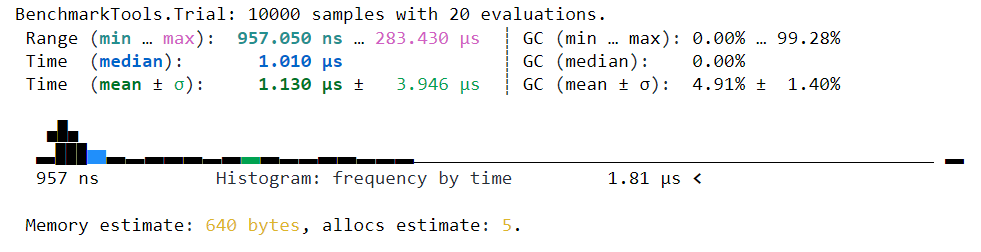
\includegraphics[width=0.9\columnwidth]{graphics/Chap10/BenchmarkAutoDiff.png}

\begin{lstlisting}[language=Julia,style=mystyle]
# Benchmarking Finite Differences

@benchmark FiniteDiff.finite_difference_jacobian(h3, x0)
\end{lstlisting}
\textbf{Output} 

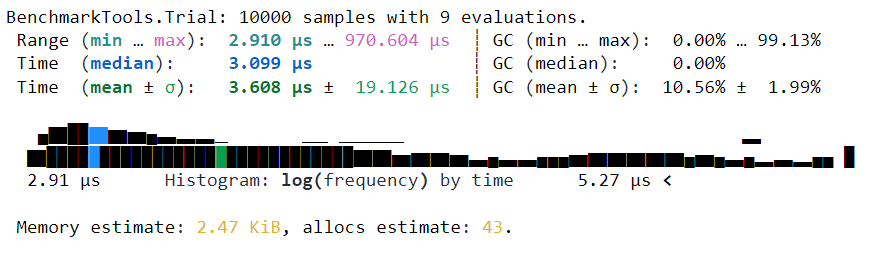
\includegraphics[width=0.9\columnwidth]{graphics/Chap10/BenchmarkFiniteDiff.png}

\begin{lstlisting}[language=Julia,style=mystyle]
# Benchmarking Symbolic Differentiation

@variables x1, x2, x3
h3s = [ x1^3*cos(x2) + x2^2*sin(x1)^2; log(3x3) ]

@benchmark begin
    dh3 = Symbolics.derivative(h3s, x)
    substitute.(dh3, (Dict(x1=>x0[1], x2=>x0[2], x3=>x0[3]),))
end

\end{lstlisting}
\textbf{Output}

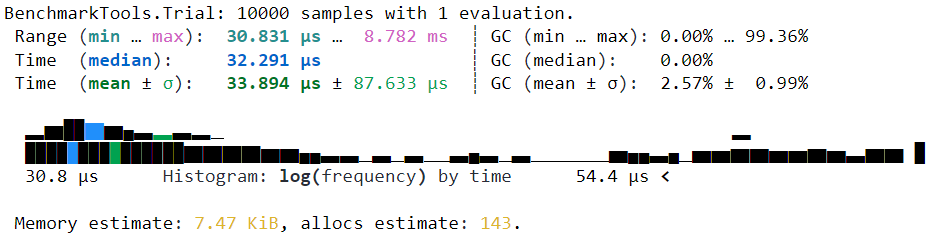
\includegraphics[width=0.9\columnwidth]{graphics/Chap10/BenchmarkSymbolicDiff.png}

\vspace*{.2cm}

\begin{tcolorbox}[title = {\large \bf Summary}]
Automatic Differentiation is the fastest, followed by Finite Differences, and Symbolic Differentiation is the slowest! And it's not even close!
\begin{itemize}
    \item Automatic Differentiation: (median): 1.010 $\mu$s 
    \item Finite Differences: (median): 3.099 $\mu$s 
    \item Symbolic Differentiation: (median): 32.291 $\mu$s 
\end{itemize}
\end{tcolorbox}

% \begin{lstlisting}[language=Julia,style=mystyle]

% \end{lstlisting}
% \textbf{Output} 
% \begin{verbatim}

% \end{verbatim}

% \begin{lstlisting}[language=Julia,style=mystyle]

% \end{lstlisting}
% \textbf{Output} 
% \begin{verbatim}

% \end{verbatim}

% \begin{lstlisting}[language=Julia,style=mystyle]

% \end{lstlisting}
% \textbf{Output} 
% \begin{verbatim}

% \end{verbatim}

% \begin{lstlisting}[language=Julia,style=mystyle]

% \end{lstlisting}
% \textbf{Output} 
% \begin{verbatim}

% \end{verbatim}

% \begin{lstlisting}[language=Julia,style=mystyle]

% \end{lstlisting}
% \textbf{Output} 
% \begin{verbatim}

% \end{verbatim}